\section{Methods}
\label{sec:methods}

We pair controlled simulations with prospective and historical Polymarket questions
\citep{gentzel2019case,polymarket2026docs}. Simulations isolate information sources;
the market studies test evidence use on open questions and accuracy on held-out,
resolved events. Contrasts are paired by question or episode. For trained models,
uncertainty is propagated first across seeds and then across episodes within seed.


\subsection{Experiment 1: Evidence-Selective Updating}
\label{sec:methods-exp1}

We sample 100 binary markets in politics, government, elections, economics, technology, and
geopolitics, each open at collection, 14--180 days from resolution, and with at
least \$1,000 in lifetime USD volume. We report three
hosted API systems \citep{openai2026gpt54,anthropic2026claude48,deepseek2026v4}
and six scale-valid Qwen~2.5 or Llama-family open-weight models
\citep{qwen2025qwen25,grattafiori2024llama}; Appendix~\ref{app:record-processing}
retains one mixed-scale deployment for compliance diagnostics.

Agents return an event model and $P(H_1)$ (YES), $P(H_2)$ (NO), with headline
forecast $\hat p=P(H_1)$. With search then disabled, they receive nine generated
packets per market---three pro-$H_1$, three anti-$H_1$, three topical but
orthogonal---giving 30,094 valid updates. The prompt carries one packet field, the
snippet text; every other field is withheld and read only at scoring
(Appendix~\ref{app:exp1-withholding}).

We report three measures. \textbf{Abstention} is the share of orthogonal
updates returning the displayed prior unchanged; \textbf{sensitivity} divides mean
absolute directional by orthogonal movement among updates that moved at all. Both
ask whether a model discriminates probative from topic-matched evidence. \textbf{Evidence--Hypothesis Consistency
(EHC)} is directional correctness for stated $P(H_1)$ among updates of at least 3
points and asks whether the forecast moves the predicted way. Appendix~\ref{app:exp1-alternatives}
gives lexical and human comparisons for packet-direction recovery and alternative
selectivity estimands. Figure color bands use
sensitivity cutpoints $2.5,4,6$ and EHC cutpoints $.90,.95,.98$. Intervals use
20,000 market-clustered resamples retaining all packets and repeated initial runs
(Appendix~\ref{app:exp1-threshold-robustness}). Eight reviewers judged 18
balanced packets against the frozen direction key, matching it on 75.0\%;
Appendix~\ref{app:exp1-limitations} gives the tally, the disclosed
post-inspection exclusion, and item-level judgments.


\begin{figure}[!ht]
\centering
% The exported figure carries ~14.5pt of blank canvas below its last box;
% trim most of it so the caption sits closer than the export padding allows.
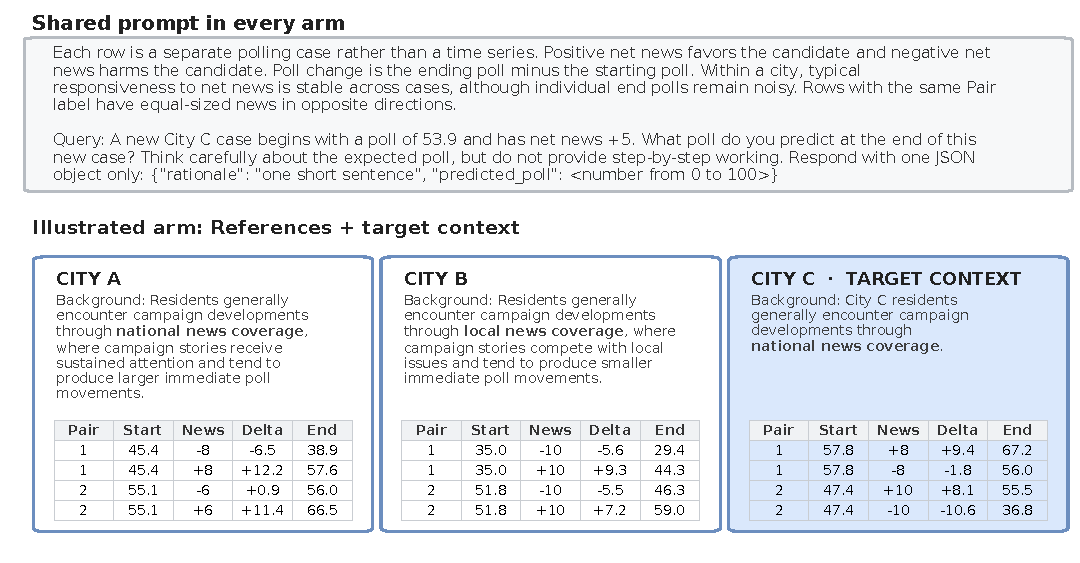
\includegraphics[width=\linewidth,trim=0 10pt 0 0,clip]{figures/exp2_coin_city_prompt_arms.pdf}
\caption{\textbf{Coin City prompt and information arms.} Every arm receives the
instructions and query shown. The illustrated episode ($k=4$) additionally provides
City A/B references and City C's qualitative context. The no-context and
opposite-context arms change only the City C sentence.}
\label{fig:coin-city-prompts}
\end{figure}

\subsection{Experiment 2: Context-Guided Relationship Selection}
\label{sec:methods-stage2}

\label{sec:methods-coin-city}

Each Coin City episode describes three cities with stable but unobserved poll
responses to news. City A and City B provide reference cases; City C provides up to
four observations and a one-sentence description naming a response regime. The
reference descriptions state which regime responds more strongly, but no prompt
states a coefficient.

We generate 250 independent episodes. For city $j$ in episode $i$,
\begin{equation}
  \Delta p_{ij}=g_jx_{ij}+\epsilon_{ij},
  \qquad \epsilon_{ij}\sim\mathcal N(0,5^2),
  \label{eq:coin-city-dgp}
\end{equation}
where $x_{ij}$ is signed net news, and strong and weak cities draw
$g_j\sim\mathcal N(0.90,0.03^2)$ and $g_j\sim\mathcal N(0.25,0.03^2)$. Each
reference city provides four cases in matched equal-and-opposite news pairs. A
query asks for City C's ending poll after news
$x\in\{-10,\ldots,-4,4,\ldots,10\}$, given $k\in\{0,1,2,3,4\}$ City C cases.

Five prompt arms vary the evidence available: target cases alone; reference cases
without City C context; references with the correct City C context; references with
the opposite context label; and an arbitrary-label arm replacing national/local
with \texttt{KIV}/\texttt{ZOR}, whose higher-response mapping changes by episode
and must be recovered from the reference cases. Paired arms share the same episode
and query values; the correct- and opposite-context prompts differ only in City C's
context sentence. Every arm reuses an episode bank under a manifest hashed before model calls
(Figure~\ref{fig:coin-city-prompts}). An open-weight activation audit reuses the
semantic and arbitrary-label arms' correct, absent, and inverted prompts and patches
the label tokens. Appendix~\ref{app:coin-city} gives full design and execution
details.

Claude Opus~4.8, Claude Opus~5, GPT-5.6, DeepSeek-V4-Pro, Kimi K3, and Gemini 3.6
Flash are evaluated on every frozen episode, evidence depth, and four semantic arms:
30,000 attempts in total. The arbitrary-label analysis extends the roster to 15
systems at $k=0$ and evaluates open-weight scale families. Forecast MAE is measured against the noise-free expectation
$p_0+g_Cx$; the forecast-implied response $\hat g=(\hat p-p_0)/x$ is reported as
MAE and as across-episode correlation with $g_C$.

A deterministic analogical benchmark uses the cue to choose City A or B, fits that
reference by through-origin OLS, and refits as City C cases arrive
(Appendix~\ref{app:coin-city-analysis}). Paired intervals use 2,000 episode
bootstrap samples \citep{efron1979bootstrap}.

\subsection{Experiment 3: Controlled Relationship Transfer}
\label{sec:methods-stage3}

\label{sec:methods-exp3-synthetic}

% Compact inline orientation graphic for the Experiment 3 transfer design: a 2x2
% grid crossing generative mechanism (rows) with surface domain (columns).
%
% Row cards carry the mechanism detail: a two-node vs three-node graph with the
% mediator drawn hollow (it is never named to the model) and a persistence loop,
% plus the six-period impulse response on labelled axes. Bar heights are the
% normalised responses to a unit shock under worlds.transition at the midpoint of
% each sampling band (direct: gain .57; mediated: gain .57, rho .61, phi .30,
% lambda .81), i.e. A = (1, 0, 0, 0, 0, 0) and B = (.81, .74, .52, .34, .21, .13).
%
% Geometry note: cards have fixed dimensions and every label is a single line
% with no text width, so nothing can rewrap into a neighbour.
% Callers may set \transfergridlines to match the paragraph they anchor this
% to; wrapfig cannot wrap a section heading, so the count must not overrun it.
\providecommand{\transfergridlines}{13}
\begin{wrapfigure}[\transfergridlines]{r}{0.48\textwidth}
\vspace{-0.8em}
\centering
\definecolor{miniCityFill}{HTML}{E8F2FB}
\definecolor{miniCityEdge}{HTML}{4F7EA8}
\definecolor{miniHarborEdge}{HTML}{3F8E82}
\definecolor{miniTestFill}{HTML}{E7F4EA}
\definecolor{miniTestEdge}{HTML}{6FA97F}
\definecolor{miniTestChip}{HTML}{5E9470}
% Coin discs reuse Figure 1's yellow pair exactly -- the fill and stroke of its
% NAIVE box -- rather than the saturated gold used before. Figure 1's other warm
% pair (#FFE6CC on #D79B00, its FREQUENTIST box) is the orange one and is not
% used here. The glyph inside each disc still carries its domain colour.
\definecolor{miniCoinFill}{HTML}{FFF2CC}
\definecolor{miniCoinRim}{HTML}{D6B656}
\definecolor{miniMute}{HTML}{8A93A3}
\definecolor{miniInk}{HTML}{3F4550}
\definecolor{miniBar}{HTML}{7C93AD}
% Coin City: a skyline stamped into a coin.
\newcommand{\coincity}[2]{%
  \begin{scope}[shift={(#1,#2)},scale=0.70]
    \fill[miniCoinFill] (0,0) circle (.37);
    \draw[miniCoinRim,line width=.75pt] (0,0) circle (.37);
    \fill[miniCityEdge] (-.23,-.18) rectangle (-.10,.04);
    \fill[miniCityEdge] (-.07,-.18) rectangle (.07,.16);
    \fill[miniCityEdge] (.10,-.18) rectangle (.24,.09);
    \draw[miniCityEdge,line width=.65pt] (-.27,-.19)--(.27,-.19);
  \end{scope}}
% Coin Harbor: a small vessel and waves stamped into a coin.
\newcommand{\coinharbor}[2]{%
  \begin{scope}[shift={(#1,#2)},scale=0.70]
    \fill[miniCoinFill] (0,0) circle (.37);
    \draw[miniCoinRim,line width=.75pt] (0,0) circle (.37);
    \fill[miniHarborEdge] (-.24,-.05)--(.24,-.05)--(.15,-.18)--(-.15,-.18)--cycle;
    \draw[miniHarborEdge,line width=.7pt]
      (-.01,-.05)--(-.01,.15)--(.15,.02)--(-.01,.02);
    \draw[miniHarborEdge,line width=.55pt]
      (-.26,-.24)..controls(-.18,-.19)and(-.10,-.29)..(-.02,-.24)
      ..controls(.06,-.19)and(.14,-.29)..(.26,-.24);
  \end{scope}}
% Impulse response on labelled axes: response (Delta y) against period (t).
\newcommand{\impulse}[3]{% #1 = axis corner x, #2 = baseline y, #3 = bar heights
  \draw[-{Stealth[length=2.6pt,width=2.2pt]},draw=miniInk!65,line width=.5pt]
    (#1,#2) -- (#1,#2+0.40);
  \draw[-{Stealth[length=2.6pt,width=2.2pt]},draw=miniInk!65,line width=.5pt]
    (#1,#2) -- (#1+0.72,#2);
  \node[anchor=south,font=\sffamily\scriptsize,text=miniInk,inner sep=1pt]
    at (#1,#2+0.40) {$\Delta y$};
  \node[anchor=west,font=\sffamily\scriptsize,text=miniInk,inner sep=1.5pt]
    at (#1+0.72,#2) {$t$};
  \foreach \i/\h in {#3}{%
    \fill[miniBar] (#1+0.055+\i*0.105,#2) rectangle (#1+0.055+\i*0.105+0.070,#2+\h);}}
\resizebox{\linewidth}{!}{%
\begin{tikzpicture}[
  x=1cm, y=1cm,
  cell/.style={rounded corners=3pt, minimum width=1.95cm, minimum height=1.25cm,
    line width=.6pt, inner sep=0pt},
  traincell/.style={cell, draw=miniCityEdge, fill=miniCityFill},
  heldcell/.style={cell, draw=miniTestEdge, fill=miniTestFill,
    dash pattern=on 1.9pt off 1.5pt},
  rowcard/.style={rounded corners=3pt, minimum width=2.60cm,
    minimum height=1.25cm, inner sep=0pt, draw=miniMute!30, fill=black!3,
    line width=.5pt},
  dname/.style={anchor=south, font=\sffamily\bfseries\scriptsize},
  rname/.style={anchor=center, font=\sffamily\scriptsize, text=miniInk},
  note/.style={anchor=center, font=\sffamily\scriptsize, text=miniInk},
  gnode/.style={circle, draw=miniInk!75, fill=white, line width=.5pt,
    inner sep=0pt, minimum size=0.26cm, font=\sffamily\tiny, text=miniInk},
  hidden/.style={gnode, draw=miniMute, fill=miniMute!14,
    dash pattern=on 1.1pt off .9pt},
  garrow/.style={-{Stealth[length=2.4pt,width=2pt]}, draw=miniInk!70,
    line width=.45pt, shorten >=.4pt, shorten <=.4pt},
  chip/.style={anchor=center, rounded corners=1.6pt, draw=none, text=white,
    inner xsep=3pt, inner ysep=1.1pt, font=\sffamily\bfseries\tiny},
]
% ---- domain marks and names ----------------------------------------------
\coincity{0.975}{2.56}
\coinharbor{3.075}{2.56}
\node[dname, text=miniCityEdge]   at (0.975,1.80) {COIN CITY};
\node[dname, text=miniHarborEdge] at (3.075,1.80) {COIN HARBOR};

% ---- Structure A: direct, one period -------------------------------------
\node[rowcard] at (-1.50,1.00) {};
\node[rname] at (-1.50,1.45) {\textbf{Structure A} direct};
\node[gnode] (ax) at (-2.51,0.82) {$x$};
\node[gnode] (ay) at (-2.07,0.82) {$y$};
\draw[garrow] (ax) -- (ay);
\impulse{-1.22}{0.62}{0/0.360, 1/0.000, 2/0.000, 3/0.000, 4/0.000, 5/0.000}

% ---- Structure B: mediated, persistent -----------------------------------
\node[rowcard] at (-1.50,-0.42) {};
\node[rname] at (-1.50,0.03) {\textbf{Structure B} mediated};
\node[gnode]  (bx) at (-2.51,-0.60) {$x$};
\node[hidden] (bm) at (-2.07,-0.60) {$m$};
\node[gnode]  (by) at (-1.63,-0.60) {$y$};
\draw[garrow] (bx) -- (bm);
\draw[garrow] (bm) -- (by);
\draw[garrow] (bm) to[out=118,in=62,looseness=4.5] (bm);
\impulse{-1.22}{-0.80}{0/0.292, 1/0.265, 2/0.188, 3/0.123, 4/0.077, 5/0.048}

% ---- the four evaluation cells -------------------------------------------
\node[traincell] at (0.975,1.00) {};
\node[heldcell]  at (3.075,1.00) {};
\node[heldcell]  at (0.975,-0.42) {};
\node[heldcell]  at (3.075,-0.42) {};

\node[chip, fill=miniCityEdge] at (0.975,1.26) {TRAINED};
\node[chip, fill=miniTestChip] at (3.075,1.26) {TEST};
\node[chip, fill=miniTestChip] at (0.975,-0.16) {TEST};
\node[chip, fill=miniTestChip] at (3.075,-0.16) {TEST};

\node[note] at (0.975,0.80) {in-distribution};
\node[note] at (3.075,0.80) {domain shift};
\node[note] at (0.975,-0.62) {structure shift};
\node[note] at (3.075,-0.62) {joint shift};
\end{tikzpicture}%
}
\vspace{-0.3em}
\caption{\footnotesize\textbf{Transfer grid.} Training uses the shaded cell;
all four are evaluated. Columns vary domain; rows vary response mechanism.}
\label{fig:exp3-transfer-grid}
\vspace{-0.9em}
\end{wrapfigure}

Training uses the direct, one-period relationship in
Equation~\ref{eq:coin-city-dgp}. Each prompt shows two complete 14-case references,
a target with $k$ observed cases, and a ten-outcome query. The episode-matched and
population-prior arms use byte-identical prompts and the same multiset of answer
keys. Matched training pairs episode $i$ with its own key $\mathbf y^\star_i$;
the control uses a fixed within-$k$ derangement $\mathbf y^\star_{\pi_k(i)}$.
This preserves the answer distribution while breaking the prompt--target link.
Neither arm supplies graph labels. A structureless diagnostic scrambles the
displayed drivers and rewards a flat response; the untrained base receives the
same evaluation prompts without training.
Table~\ref{tab:exp3-training-policies}
in Appendix~\ref{app:exp3-coin-structural} shows all four conditions on one episode.


Policies train only on Coin City under Structure~A, the direct mechanism
$x_t\to y_{t+1}$. Figure~\ref{fig:exp3-transfer-grid} crosses this trained cell
with a new surface domain (Coin Harbor), the mediated Structure~B
($x_t\to m_{t+1}\to y_{t+1}$), and both shifts together.

Evaluation crosses domain, mechanism, pathway hint, and
$k\in\{0,2,4,8\}$, yielding $1{,}440$ paired prompts; each training run contains
4,800 Coin City/Structure~A prompts. The primary estimand is population-prior
minus episode-matched response MAE under joint shift and the correct hint. We use
three Qwen3-8B seeds per arm at round 300 and average five stochastic draws within
task before a paired seed-first bootstrap. The Qwen3-4B scale replication,
structureless control, Llama-8B comparator, prompts, and parameters appear in
Appendix~\ref{app:exp3-coin-structural}.

\begin{figure}[b]
\centering
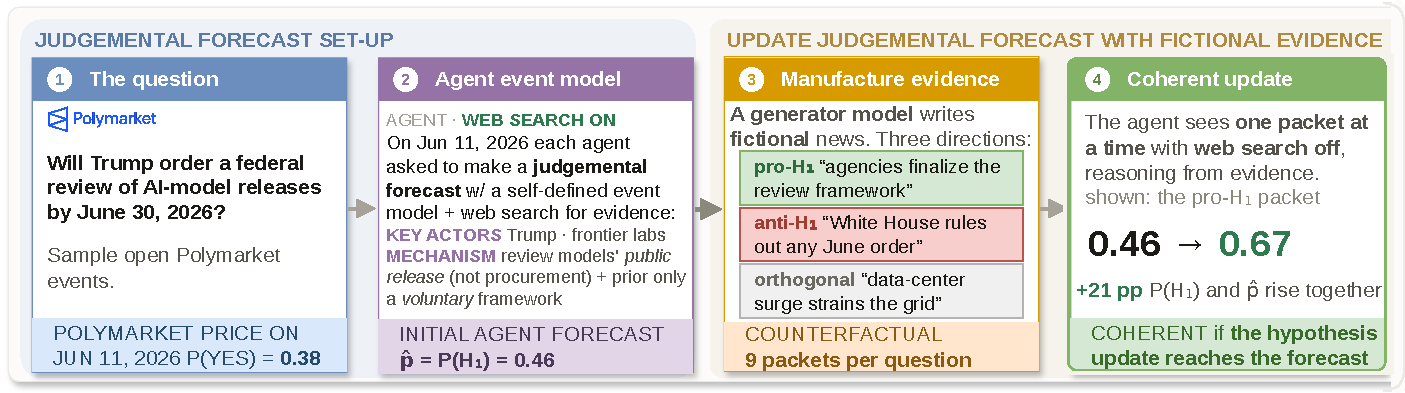
\includegraphics[width=\linewidth]{figures/exp1_protocol_four_panels.pdf}
\caption{\textbf{Prospective evidence-intervention protocol.} An agent forecasts an
unresolved question, then receives one generated evidence packet with search off.
The packet's intended direction is never shown to the agent; it is read only when
the update is scored.
Directional correctness asks whether the update follows a pro- or anti-$H_1$
packet. Selectivity compares movement under directional and orthogonal packets.
The output contract requires $\hat p=P(H_1)$, so agreement between those fields is
partly schema compliance.}
\label{fig:exp1-pipeline}
\end{figure}

\subsection{Experiment 4: Historical-Market Training and Sealed Evaluation}
\label{sec:methods-exp4-polymarket}

Resolved political, governmental, macroeconomic, and geopolitical markets are cut
off 30 days before their earliest archived terminal timestamp. Prompts retain only
the question, rules, cutoff, and genuine pre-cutoff prices. Outcomes and post-cutoff
fields are withheld. Calendar splits contain 1,736 training, 512 development, and
1,024 test markets, with no event or normalized question family shared across
splits.

We train Qwen3 and Llama checkpoints \citep{qwen2025qwen3,grattafiori2024llama} with
rank-32 LoRA \citep{hu2022lora} and Dr.~GRPO
\citep{liu2025understanding} for 300 rollout-and-update rounds (4,800 prompt
presentations) at each of three seeds. Reward is the proper score
$1-(\hat p-y)^2$ \citep{brier1950verification}; training alone supplies
gradients. Development selects no endpoint, and test data are absent from
training.

The scale comparison evaluates three-seed Qwen3 checkpoints at 1.7B, 4B, 8B, and
14B parameters and Llama checkpoints at 3B and 8B on a 318-market holdout disjoint
from all training, development, and test families. Every base and trained endpoint is
scored from five non-thinking stochastic draws. Brier intervals resample connected
event/template families \citep{brier1950verification,good1952rational}. A Qwen3-4B
evidence-updating evaluation also applies the Experiment~1 packets to the base and
final adapters. Appendix~\ref{app:exp3b-protocol} gives the censoring, checksums,
optimization, held-out evaluation, scale comparison, and revision-analysis details.
